% Results plan: five subsections, one claim each, the subheading states the finding.

\section{Results (2,250 words, five subsections)}\label{sec:results}

\role{Turn the thesis into evidence in the order a sceptic needs it: trust the object (R1), see the gap
(R2), see the fix (R3), see that clinicians agree (R4), see that it leaves the simulator (R5).}

\noindent\textbf{Rules for every subsection.} Open with the claim as a sentence; one figure; effect sizes
with 95\% CIs, $n$ in cases, the test used; the case is the unit, seeds averaged within case; method
details go to Methods.

% ---------------------------------------------------------------------------------------------
\subsection{R1. An executable clinical-policy benchmark for local agents}\label{sec:benchmark}

\role{The reader must trust the object before any result trained on it; reviewers look here for leakage
and simulator artefacts.}

\content
\begin{itemize}
\item Episode: presentation, one typed action per turn (16 tools, 12 turns), stored results.
\item Policy and reward: components, gating by diagnosis $\times$ coverage, caps 0.10 / 0.35 / 0.50;
perfect-agent check as proof of internal consistency.
\item The hook: Fig.~1e numbers (\$682 vs \$1,313; 0.95 / 0.73 / 0.50).
\item Dataset: 600 cases, 20 conditions, difficulty and setting mix; review rule and defect-class fixes;
split with two held-out conditions; leakage AUC $\approx$0.5.
\end{itemize}

\structure
\begin{enumerate}
\item Episode and tools (100 words).
\item Policy, reward, Fig.~1e (180).
\item Cases and physician review, [N] approved test policies (130).
\item Split and leakage (90).
\end{enumerate}
\textbf{Not here:} generation prompts, tool schemas, reward equations (Methods).

\artefacts
\begin{itemize}
\item \textbf{Fig.~1} (overview): a single picture of deployment, harness, policy, reward and the hook;
the paper's entry point.
\item \textbf{Fig.~2} (benchmark): case anatomy, coverage, review loop, leakage; answers ``is the
dataset sound?'' in one look.
\end{itemize}

\status{Figs.~1--2 drafted. [N] from the review server; ``held-out conditions never in training''
holds once SE-P07 is removed from train.}

\begin{figure}[p]
\centering
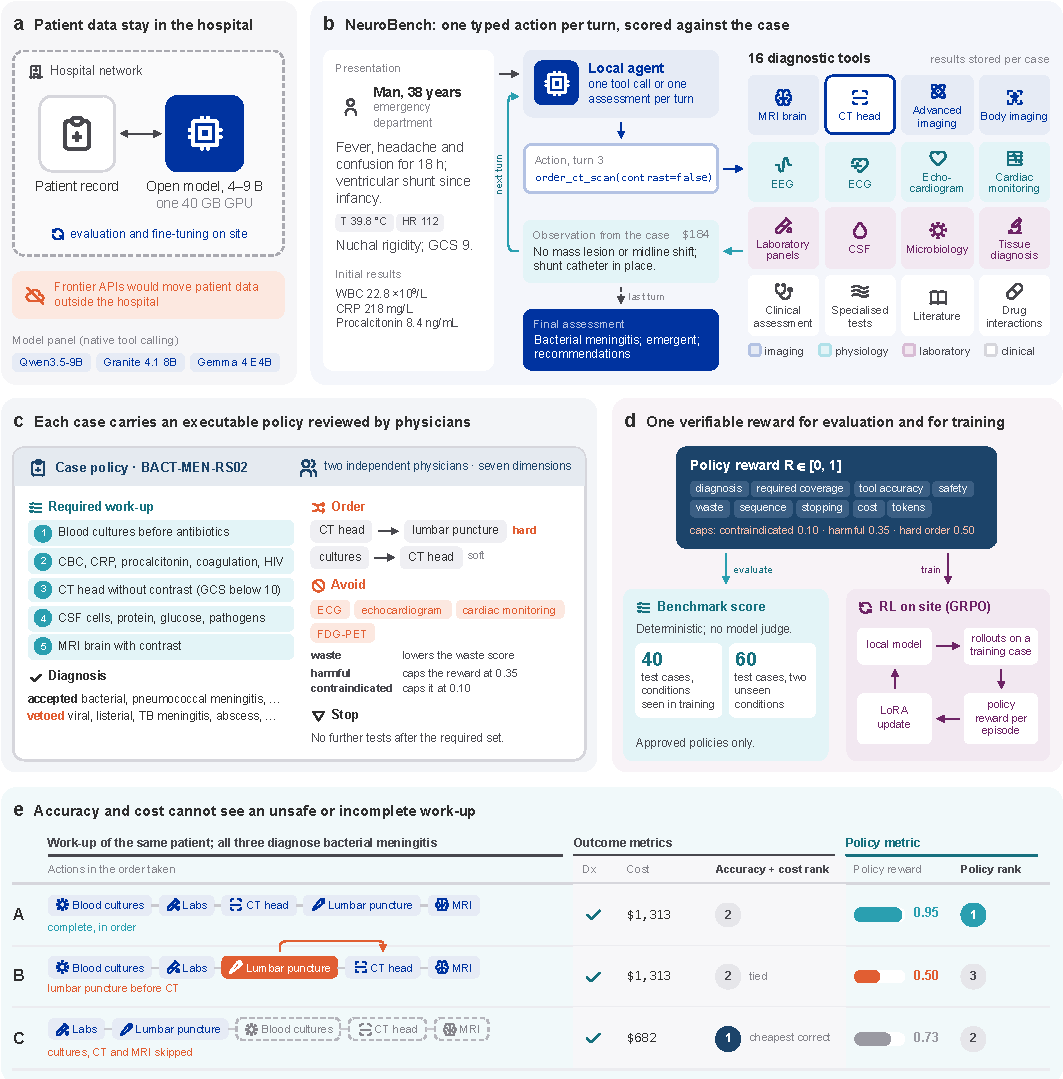
\includegraphics[width=\textwidth]{fig1.pdf}
\caption{\textbf{Draft.} Panels: \textbf{a}, local deployment; \textbf{b}, one typed action
per turn; \textbf{c}, the executable policy; \textbf{d}, the policy reward as metric and RL reward;
\textbf{e}, three work-ups, same diagnosis, opposite rankings. \emph{Why:} the whole thesis in one
figure; panel e is the hook. Legend to write ($\le$250 words), title must state the finding.}
\label{fig:overview}
\end{figure}

\begin{figure}[p]
\centering
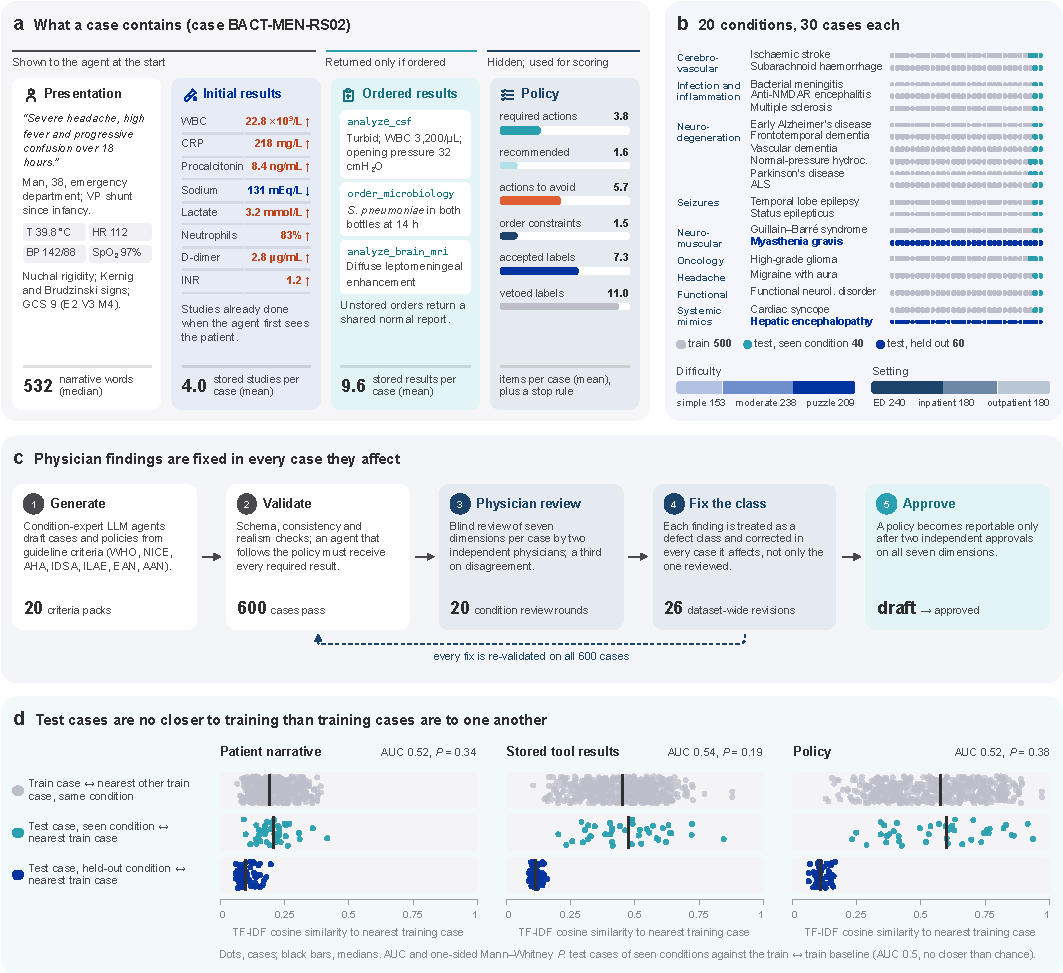
\includegraphics[width=\textwidth]{fig2.pdf}
\caption{\textbf{Draft.} Panels: \textbf{a}, what a case contains (visible, on order, hidden);
\textbf{b}, 20 conditions and the split; \textbf{c}, generation, validation, blind review, defect-class
fixes; \textbf{d}, nearest-neighbour similarity to training for narrative, results and policy.
\emph{Why:} pre-empts the dataset-quality and leakage objections. Legend to write ($\le$250 words).}
\label{fig:benchmark}
\end{figure}

% ---------------------------------------------------------------------------------------------
\subsection{R2. Outcome metrics hide unsafe work-ups and change the ranking of models}\label{sec:outcome}

\role{Claim C1 (E4). Shows the Fig.~1e example at scale: the gap is real and frequent, so training on
the outcome is a problem worth solving.}

\content
\begin{itemize}
\item Panel: Qwen3.5-9B, Granite 4.1 8B, Gemma 4 E4B $\times$ policy / direct / ReAct loops, plus two or
three frontier models.
\item Accuracy and cost vs policy reward per model.
\item Share of correct diagnoses reached with a cap triggered or required actions missing.
\item Rank agreement between outcome and policy rankings (Kendall $\tau$, bootstrap CI).
\end{itemize}

\structure
\begin{enumerate}
\item Claim and setup (80 words).
\item Correct but unsafe: rates per model (150).
\item Rankings change (120).
\item One concrete episode (50).
\end{enumerate}

\artefacts
\begin{itemize}
\item \textbf{Fig.~3}: a, accuracy vs policy reward (one point per model $\times$ loop); b, slope chart of
the two rankings; c, stacked violation types behind correct diagnoses; d, one episode. \emph{Why:}
a and b show mis-ranking, c shows what outcome hides, d makes it concrete.
\item \textbf{ED2} loop ablation: keeps loops out of the main story.
\end{itemize}

\status{To run on the frozen dataset; all earlier baselines predate scorer v2.}

\begin{figure}[p]
\centering
\figplaceholder{Fig.~3 | Outcome metrics vs the policy reward across the panel (E4)}{%
\textbf{a}, accuracy vs mean policy reward, 95\% CIs. \textbf{b}, accuracy+cost ranking vs policy
ranking, Kendall $\tau$. \textbf{c}, violations among correct diagnoses, per model. \textbf{d}, one
episode: correct diagnosis, unsafe path.}
\caption{To design after E4.}
\label{fig:panel}
\end{figure}

% ---------------------------------------------------------------------------------------------
\subsection{R3. Training on the policy reward teaches the work-up without losing accuracy}\label{sec:rl}

\role{Claims C2 and C4 (E1): the causal test of the thesis. Everything else supports this subsection,
so it gets the most words.}

\content
\begin{itemize}
\item Design: base $\to$ SFT $\to$ GRPO with two rewards that differ only in the signal (outcome =
accuracy + cost, SDBench-style; policy). Same models, data, seeds, budget.
\item Approved test split, seen and held-out conditions separately: accuracy, required coverage, safety
violations, cost, number of actions.
\item What the outcome arm learns: shortcuts (skipped cultures or imaging, invasive tests early).
\item Statistics: paired by case; Wilcoxon + paired bootstrap; McNemar for binary outcomes.
\end{itemize}

\structure
\begin{enumerate}
\item Design in two sentences, the two arms (100 words).
\item Main effect on the test split (200).
\item Held-out conditions (120).
\item Learned behaviour, with examples (130).
\item Accuracy is not paid for it; cost and tokens (50).
\end{enumerate}

\artefacts
\begin{itemize}
\item \textbf{Fig.~4}: a, training curves (train-side validation only); b, paired test results for
base, SFT, GRPO-outcome, GRPO-policy; c, same on held-out conditions; d, action sequences of both arms
on one case. \emph{Why:} b is the central number; c answers ``memorised conditions''; d shows the
mechanism (shortcuts vs work-up).
\item \textbf{ED3} seeds and CIs; \textbf{ED4} reward-weight sensitivity: the effect is not a tuning
artefact.
\end{itemize}

\status{To run. July GRPO not reportable (test split used for selection); September runs lack
evaluation and their rollouts sit only on the A100 VM.}

\begin{figure}[p]
\centering
\figplaceholder{Fig.~4 | Outcome reward vs policy reward in RL (E1)}{%
\textbf{a}, training curves of both arms. \textbf{b}, test split, paired per case: accuracy, required
coverage, violations, cost. \textbf{c}, the 60 held-out-condition cases. \textbf{d}, action sequences of
the two arms on one case.}
\caption{To design after E1.}
\label{fig:rl}
\end{figure}

% ---------------------------------------------------------------------------------------------
\subsection{R4. Physicians agree with the policy reward}\label{sec:validity}

\role{Claim C3 (E2). Without it the policy reward is our opinion; NMI reviewers will ask whether the
metric measures what clinicians value.}

\content
\begin{itemize}
\item Blinded rating of a stratified sample of episodes (model and reward hidden), fixed scale for
safety and appropriateness.
\item Spearman $\rho$ of physician scores with policy reward, accuracy+cost and an LLM judge.
\item Inter-rater agreement (Cohen or Fleiss $\kappa$).
\end{itemize}

\structure
\begin{enumerate}
\item Design (100 words).
\item Correlations, policy vs alternatives (170).
\item Agreement and disagreements (80).
\end{enumerate}

\artefacts
\begin{itemize}
\item \textbf{Fig.~5}: a, design; b, $\rho$ for the three scores with CIs; c, $\kappa$. \emph{Why:} b
is the claim; c bounds how much agreement is possible.
\end{itemize}

\status{To design and run; needs physician time. Fix sample size and protocol this week.}

\begin{figure}[p]
\centering
\figplaceholder{Fig.~5 | Blinded physician ratings vs automatic scores (E2)}{%
\textbf{a}, rating design. \textbf{b}, physician score vs policy reward, accuracy+cost, LLM judge
(Spearman $\rho$, CIs). \textbf{c}, inter-rater agreement.}
\caption{To design after E2.}
\label{fig:validity}
\end{figure}

% ---------------------------------------------------------------------------------------------
\subsection{R5. Transfer to real patient records and cost of local deployment}\label{sec:transfer}

\role{Claims C4 and C5 (E3, E5). Answers ``it only works on your simulator'' and makes the local
argument of \P1 concrete.}

\content
\begin{itemize}
\item Trained agents on MIMIC-IV neurology admissions, scored against the guideline policy and compared
with clinicians' recorded orders.
\item Latency, GPU memory and cost per case on one A100 vs frontier APIs.
\end{itemize}

\structure
\begin{enumerate}
\item Cohort and scoring (100 words).
\item Transfer results (180).
\item Deployment cost (120).
\end{enumerate}
\textbf{Fallback:} no MIMIC-IV in time $\Rightarrow$ keep deployment only, transfer becomes future work.

\artefacts
\begin{itemize}
\item \textbf{Fig.~6}: a, MIMIC-IV accuracy and adherence for base, GRPO-outcome, GRPO-policy; b,
overlap of agent orders with the policy and with clinicians; c, latency, memory, cost per case.
\emph{Why:} a and b carry C4 on real data; c carries C5.
\end{itemize}

\status{E3 waits for MIMIC-IV access (requested Oct 2026); E5 can run now.}

\begin{figure}[p]
\centering
\figplaceholder{Fig.~6 | Real records and deployment cost (E3, E5)}{%
\textbf{a}, MIMIC-IV cohort: accuracy and adherence per arm. \textbf{b}, overlap with policy and with
clinicians' orders. \textbf{c}, latency, memory, cost per case, local vs API.}
\caption{To design after E3 and E5.}
\label{fig:transfer}
\end{figure}
